\chapter{Limit Setting and Results}

\section{Introduction}

Once the event selection and background estimation procedure have been defined
and the data has been collected one needs to determine the limit on the cross
section of a possible SUSY signal (according to a specific model) or, if a 
discovery has been made, the significance of that discovery. In the present case 
no discovery has been made so a limit on the cross section must be found. There 
are various statistical procedures for doing this and no consensus on the best 
method. Here the CLs method is used. The CLs method is widely used in the field 
of particle physics. \\

A likelihood function must be defined. The likelihood is the probability of 
the data being observed given a model. This encompasses the statistical 
uncertainties on the expected number of events as well as the systematic 
uncertainties associated with the background estimation and signal prediction 
(e.g. luminosity measurement and jet energy scale uncertainty). Parameters in 
the likelihood include the parameter of interest on which we wish to set a limit 
-- the amount of signal in this case -- in addition to nuisance parameters 
associated with the systematic uncertainties. \\

The goal is to find a confidence interval for the parameter of interest based
on the likelihood. This gives an upper limit on the size of a possible SUSY 
signal at a given confidence level. An exclusion plot with the expected limit
and the observed limit is given for the GMSB models considered here in squark 
mass vs gluino mass parameter space. The exclusion plot for another CMS analysis
of the same dataset looking at the same SUSY models is shown for comparison.

\section{Likelihood Function}

The likelihood function is the probability of observing the data given the
model. There is a statistical component to the likelihood based on the number of
events we can expect given a model prediction. The statistical component follows
a poisson distribution. There are also systematic uncertainties based on how 
well the signal and background are predicted. These contribute a gaussian
component to the likelihood. \\

Let: 
\begin{itemize}
\item $b$ = Estimated number of background events;
\item $s$ = Number of expected signal events according to the model being
tested;
\item $n$ = Number of events observed.
\end{itemize}

Considering only the statistical uncertainty on the expected number of events, 
which follows a Poisson distribution, the likelihood for the background only 
hypothesis is given by Equation \ref{eq:Poisson_Likelihood_BackgroundOnly}.

\begin{equation}
L_{b} = p(n|b) = \frac{b^{n}e^{-b}}{n!} 
\label{eq:Poisson_Likelihood_BackgroundOnly}
\end{equation}

And for the signal plus background hypothesis the likelihood is given by Equation
\ref{eq:Poisson_Likelihood_SignalPlusBackground}.

\begin{equation}
L_{s+b} = p(n|s+b) = \frac{(s+b)^{n}e^{-(s+b)}}{n!} 
\label{eq:Poisson_Likelihood_SignalPlusBackground}
\end{equation}

The number of signal events can be written as:
\begin{equation}
s = f\epsilon\sigma L
\label{eq:fsig}
\end{equation}

This is the same as Equation \ref{eq:Number_of_signal_events} for the number of 
signal events, except that a signal strength factor, $f$, has been added. $f$ is 
the parameter of interest on which we are seeking to set a limit. The likelihood 
for the signal plus background hypothesis can now be written as Equation 
\ref{eq:SignalPlusBackground_Rewritten}. 

\begin{equation}
L_{s+b}(f) = \frac{(f\epsilon \sigma L + b)^{n} e^{-(f\epsilon \sigma L + b)}}{n!} 
\label{eq:SignalPlusBackground_Rewritten}
\end{equation}

Systematic uncertainties are introduced to the likelihood by allowing the 
parameters in the likelihood ($b$, $\epsilon$, $\sigma$ and $L$) to vary 
according the their uncertainties. These parameters are called nuisance 
parameters. To implement this, gaussian terms are added to the likelihood with 
mean equal to the estimated value and sigma equal to the uncertainty. This 
allows them to vary away from their estimated value, but the gaussian constrains 
them according to their uncertainty by paying a penalty in the likelihood. For 
example, the integrated luminosity was measured to be $1.100\pm0.044 
\unit{fb^{-1}}$ so a gaussian term with mean 1.100 and sigma 0.044 is added to 
the likelihood. Equation \ref{eq:Full_Likelihood} shows the full likelihood 
function, including nuisance parameters. 

\begin{eqnarray}
L_{s+b}(f; \theta_{b}, \theta_{\epsilon}, \theta_{\sigma}, \theta_{L}) &=&
\frac{(\theta_{\epsilon}\theta_{\sigma}\theta_{L}+\theta_{b})^{n}e^{-(\theta_{\epsilon}\theta_{\sigma}\theta_{L}+\theta_{b})}}{n!}
\nonumber \\
&\cdot&
\frac{1}{\sqrt{2\pi}\sigma_{b}}e^{-\frac{1}{2}\left(\frac{\theta_{b}-b}{\sigma_{b}}\right)^{2}}
\nonumber \\
&\cdot&
\frac{1}{\sqrt{2\pi}\sigma_{\epsilon}}e^{-\frac{1}{2}\left(\frac{\theta_{\epsilon}-\epsilon}{\sigma_{\epsilon}}\right)^{2}}
\nonumber \\
&\cdot&
\frac{1}{\sqrt{2\pi}\sigma_{\sigma}}e^{-\frac{1}{2}\left(\frac{\theta_{\sigma}-\sigma}{\sigma_{\sigma}}\right)^{2}}
\nonumber \\
&\cdot& 
\frac{1}{\sqrt{2\pi}\sigma_{L}}e^{-\frac{1}{2}\left(\frac{\theta_{L}-L}{\sigma_{L}}\right)^{2}} 
\label{eq:Full_Likelihood}
\end{eqnarray}

The likelihood is used in the CLs method to find the upper limit on the
parameter of interest, $f$.

\section{CLs}

The CLs method is used to determine the confidence interval for the parameter of
interest, $f$. The method is widely used within particle physics: it was used at
the Tevatron for the Higgs limit \cite{cls_tevatron} and at the LHC for the 
Higgs limit \cite{cls_lhc} and SUSY searches \cite{ra1}. The CLs method profiles
the nuisance parameters to incorporate systematic uncertainties in the limit. \\

The procedure for finding the confidence interval using CLs is:

\begin{itemize}
\item Construct a likelihood function. Equation \ref{eq:Full_Likelihood} in this 
case.
\item Construct a test statistic $q_{f}$ for performing a hypothesis test. There 
are various possible choises for the this, here the profile likelihood ratio is
used (Equation \ref{eq:Test_Statistic}).
\begin{equation}
q_{f} =
\frac{L_{s+b}(f;\hat{\boldsymbol\theta})}{L_{b}(0;\hat{\boldsymbol\theta})}
\label{eq:Test_Statistic}
\end{equation}
\item Step through the possible values of the parameter of interest, $f$.
\item Consider two hypotheses: the signal + background hypothesis and the
background only hypothesis. For each hypothesis generate pseudo data according 
to the likelihood. Call the generated data ``MC toys''.
\item Calculate the the p-values:
\begin{eqnarray}
CLsb &=& P(q_f \geq q_f^{obs}|\mbox{signal + background}) \label{eq:alpha} \\
CLb &=& P(q_f \geq q_f^{obs}|\mbox{background only}) \label{eq:1minusbeta}
\end{eqnarray}
These are the fraction of MC toys for which the test statistic is greater than
the observed value given the signal + background hypothesis (Equation
\ref{eq:alpha}) and given the background hypothesis (Equation 
\ref{eq:1minusbeta}).
\item Construct CLs as a ratio of p-values (Equation \ref{eq:CLs}). This cannot 
be interpreted as a p-value itself. It gives an idea of how much more probable 
to observe the data given the signal + background hypothesis than the background 
only hypothesis.
\begin{equation}
CLs = \frac{CLsb}{CLb}
\label{eq:CLs}
\end{equation}
\item Those values of $f$ for which $CLs < \nu$ are excluded at a confidence
level (CL) of $1-\nu$. Here the CL is taken to be 95\%. The upper limit on $f$ 
at 95\% CL is the value of $f$ for which $CLs = 0.05$.
\end{itemize}

The CLs method is used to calculate the upper limit on $f$ for each point in the
parameter space. Figure \ref{fig:limit} shows the upper limit on $f$ in the
squark mass vs gluino mass plane for the 441 points in the grid.

\begin{figure}
\begin{center}
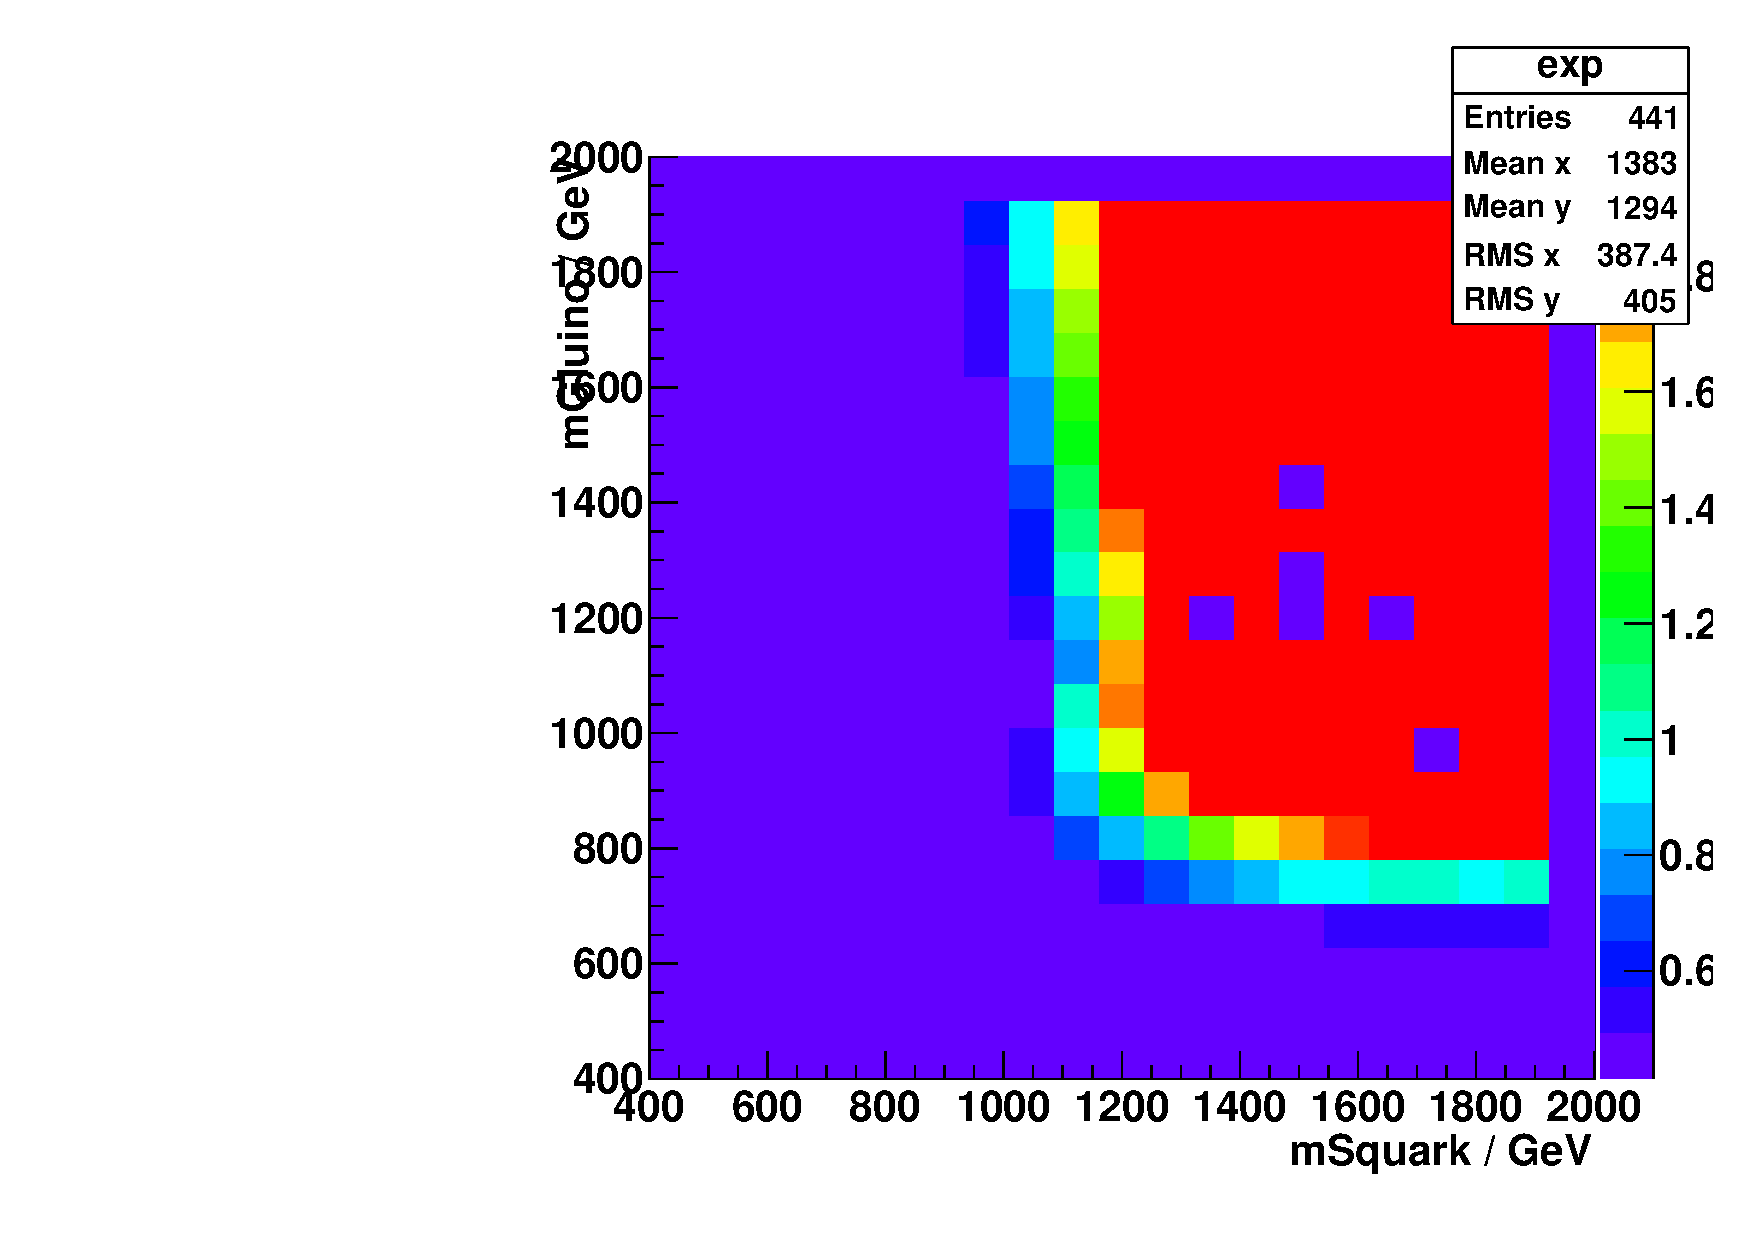
\includegraphics[width=0.8\textwidth]{ExpectedLimit.pdf}
\end{center}
\caption{The expected upper limit on $f$ in the squark mass vs gluino mass plane 
using the CLs method. }
\label{fig:limit}
\end{figure}

\section{Interpolation and Smoothing}

The grid of SUSY parameter points is rather coarse giving a jagged exclusion
line. To make a smooth limit an interpolation is performed between the points 
on the grid to make a finer grid with more points in the parameter space. The 
upper limit on $f$ is taken to vary linearly between points on the grid. Figure
\ref{fig:interpolation} shows the finer grid after linear interpolation between
the points. The resulting exclusion line is still slightly jagged due to the
finite number of points in the interpolation. To smooth the line each point
along the line is replaced by a moving average which is the mean of the closest 
five points.

\begin{figure}
\begin{center}
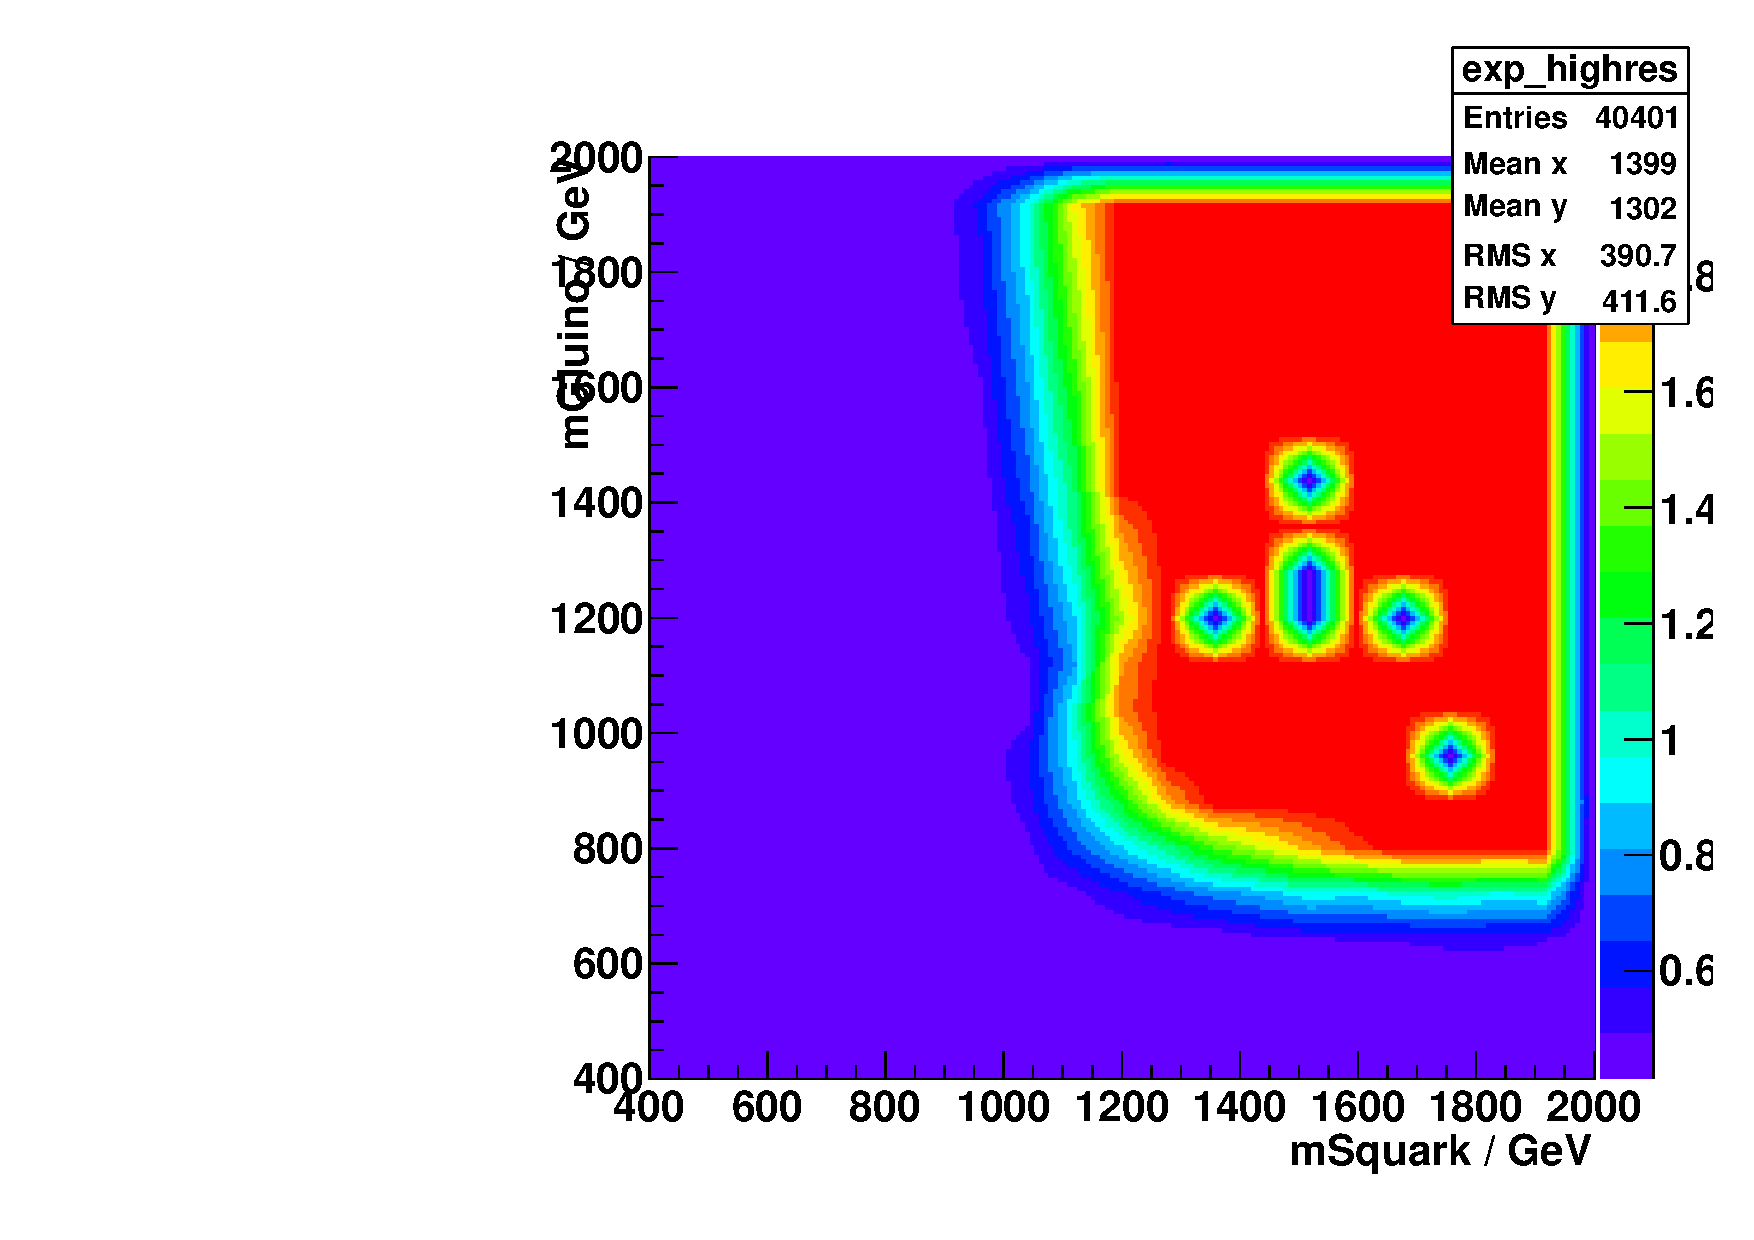
\includegraphics[width=0.8\textwidth]{ExpectedLimit_HighRes.pdf}
\end{center}
\caption{The expected upper limit on $f$ in the squark mass vs gluino mass plane 
after a linear interploation between the points. }
\label{fig:interpolation}
\end{figure}

\section{Expected and Observed Limit}

An expected limit without looking at the data can be calculated. Pseudo data is
generated using the background model. An expected limit is calculated using any
of the above methods using the pseudo data as if it were data. \\

Many sets of pseudo data are generated and a limit on the cross section of a 
possible SUSY signal is calculated for each. An expected limit can be drawn on 
the SUSY parameter space by linking those parameter points for which the signal 
can be excluded at 95\% confidence level in half of the pseudo experiments. The 
$1 \sigma$ band, a line linking the parameter points where the signal is 
excluded for 68\% of the pseudo experiments, is also drawn. \\

Figure \ref{fig:finallimit} shows the final limit plot at 95\% CL with the
expected limit, the $\pm1$ sigma band and the observed exclusion limit. The
exclusion limit from another CMS analysis \cite{ra3} looking at the same signal 
model is also shown for comparison. \\

The limits on GMSB from previous experiments such as ALEPH \cite{aleph}, CDF
\cite{cdf} and D0 \cite{d0} are concerned with electroweak production rather than 
strong production. A direct comparison is difficult since the results are 
interpreted in a different parameter space, but these experiments have a much 
lower reach in terms of squark and gluino mass due to the lower $\sqrt{s}$. \\

The limit presented here excludes more parameter space than the RA3 limit
(Figure \ref{fig:finallimit}) at high gluino mass and less parameter space at 
high squark mass. This makes sense because the RA3 search looks at the
$\gamma\gamma+\MET$ signature which is better in a cleaner environment with
fewer jets, but worse in an environment with more jets because a photon can
get lost. Parameter points with high gluino mass tend to have more jets.

\begin{figure}
\begin{center}
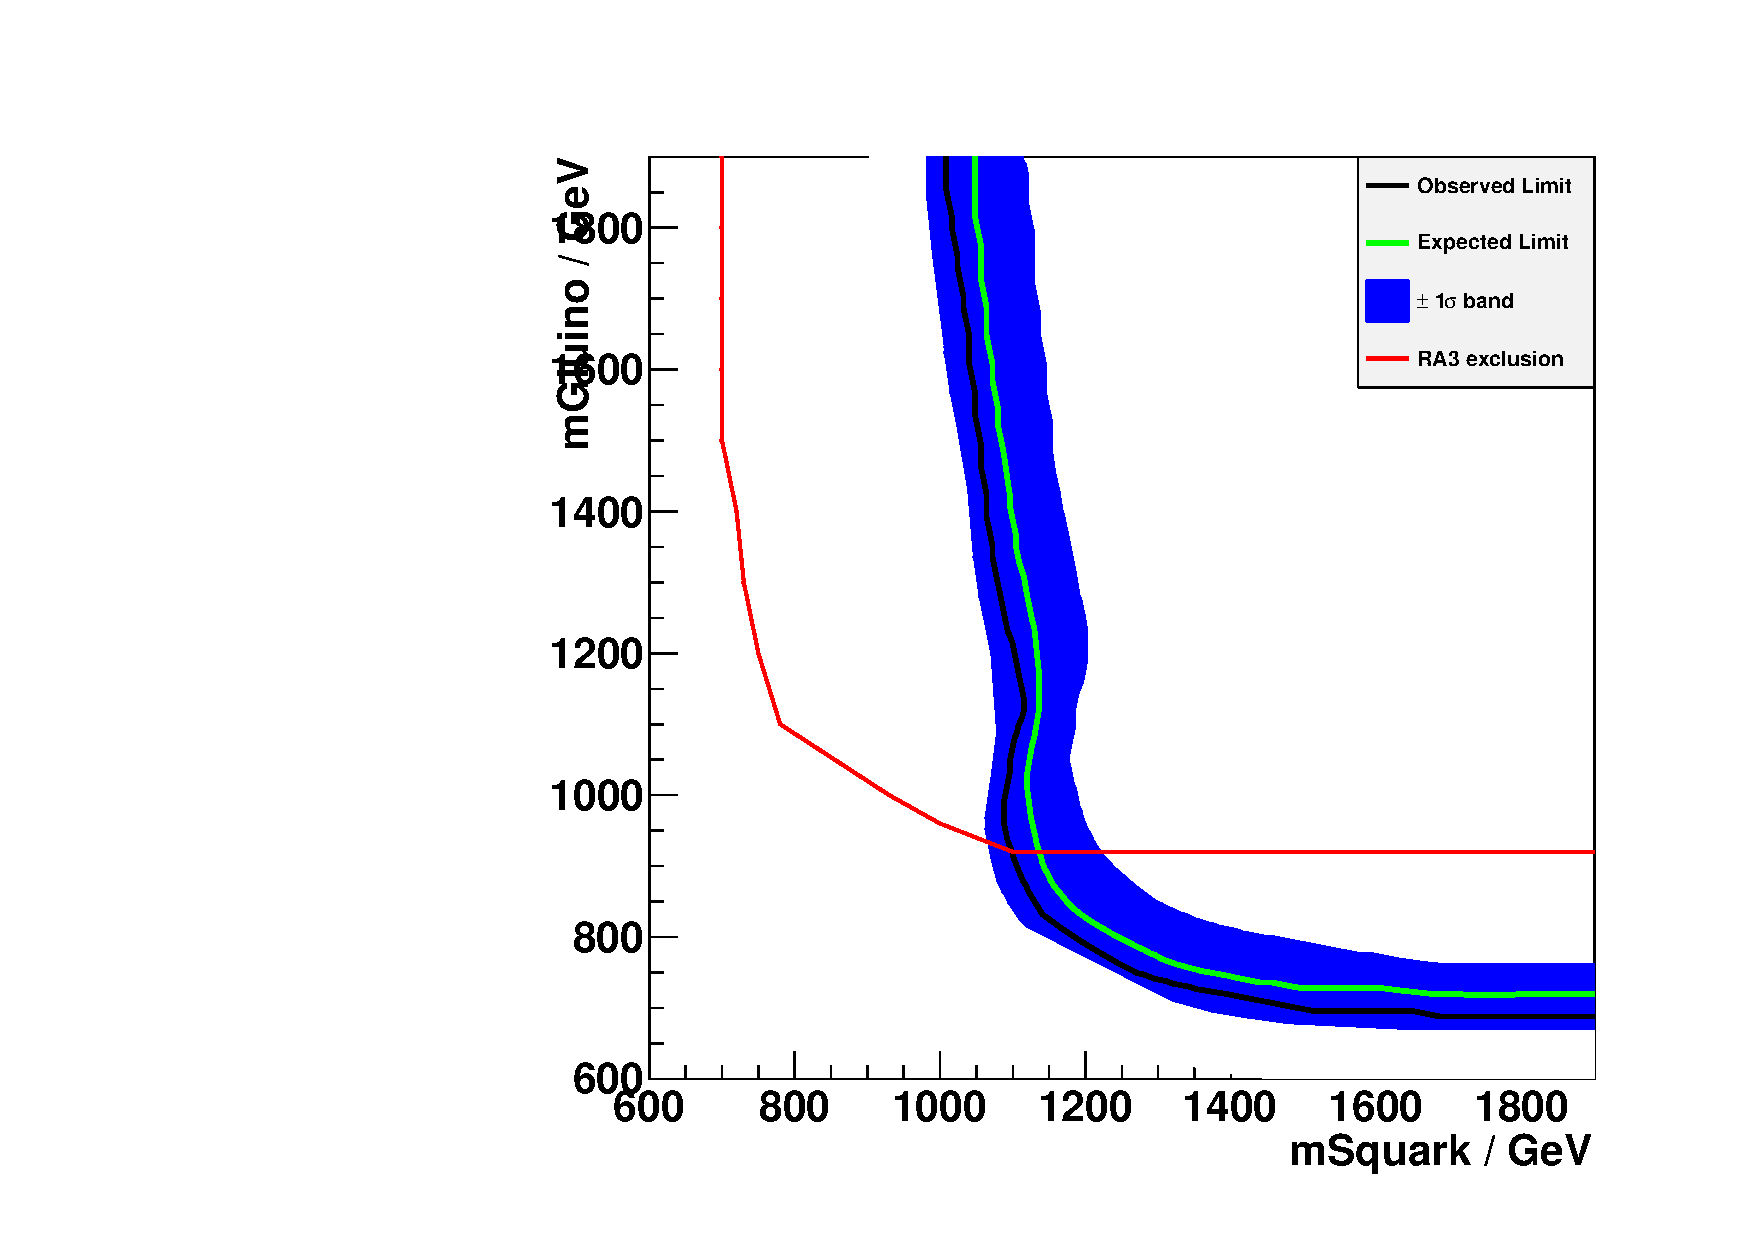
\includegraphics[width=0.8\textwidth]{graph.pdf}
\end{center}
\caption{The expected upper limit on $f$ in the squark mass vs gluino mass plane 
after a liner interploation between the points. }
\label{fig:finallimit}
\end{figure}
